% !TEX root       = ./type_name.tex
% !TEX program    = pdflatex
% !TEX encoding   = utf-8
% !TEX spellcheck = de_DE_frami
%=======================================================================
\chapter{Evaluation}\label{ch:Evaluation}
To evaluate whether the developed application works as intended, it is tested against the testbed setup as shown in this figure below. This chapter also discusses about the performance of RYU controller and Open vSwitch against the application’s performance.

  \begin{figure}
	\centering
	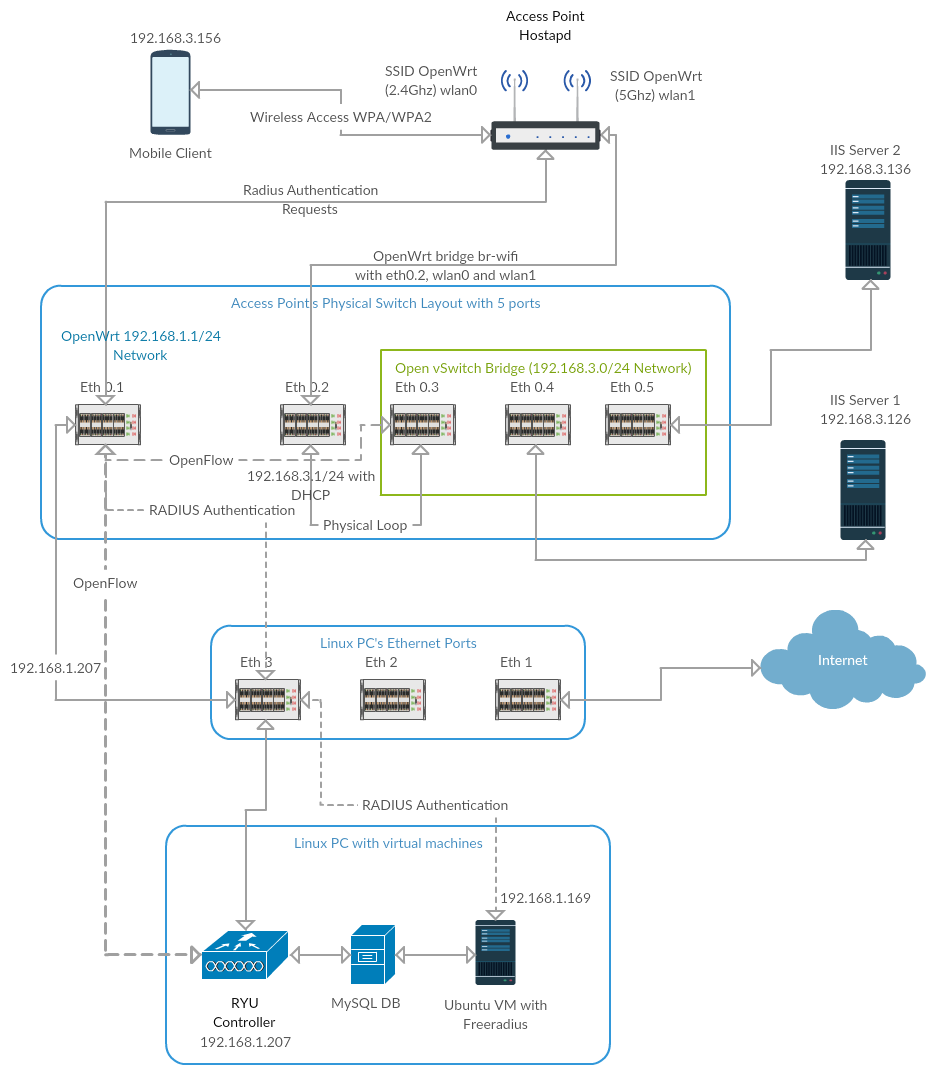
\includegraphics[width=1.0\linewidth]{Physical-Layout}
	\caption {Physical Layout of the Test Environment}
	\label{fig:test-layout}
	\vspace{-10pt}
  \end{figure}

\section{Testbed Description}
The image \ref{fig:test-layout} shows how the environment for testing is set up. Each section is explained below in details about the configuration and how each port functions against the devices connected to it.

The Mobile Client is a Samsung Nexus Android phone and the second device used is also an Android device capable of associating with a network via 802.1x. The Access Point is a TP-Link WDR4300 WLAN router capable of dual band wireless access. This is convenient for the project as each band can be associated to a separate SSID (OpenWrt and OpenWrt 5G) that clients can connect with using different credentials.

The physical switches of the access point is shown separately for a better view. The router consists of five Ethernet ports including one WAN port. The WAN port is configured to work as a LAN access port for management access from the Linux PC. The Ethernet ports Eth0.1 and Eth0.2 are connected using the OpenWrt br-lan bridge. The port Eth0.2 is connected to Eth0.3 using a physical loop cable since internal looping was not possible due to constrains in the board design.

The bridge managed by Open vSwitch consist of the ports from Eth0.3 to Eth0.5 and includes a DHCP that provides a separate 192.168.3.1 network and gateway for all the devices connect to these ports. The ports Eth0.4 and Eth0.5 are connected to an IIS server running on a Windows 7 and Windows 10 operating systems respectively on two separate Laptops. Each of these server machines are connected to the OVS managed ports on a separate network, the Windows 7 machine is connected using 192.168.3.126 and the Windows 10 with 192.168.3.136.

The Linux PC on the other hand, consist of three physical network interface cards numbered in order from Eth1 to Eth3. It runs Edubuntu, a flavor of Ubuntu designed for educational use. The port Eth1 is connected to the internet and the port Eth3 is connected to the router which is associated with an IP 192.168.1.207. The PC also hosts a Virtual Box Ubuntu VM running Freeradius, the virtual network adapter is bridged with Eth3 port in the PC and has the IP 192.168.1.169. The application MySQL and RYU controller reside in the PC and are associated to the PC’s IP.
%\begin{itemize}
%	\item The Mobile Client used here is a Samsung Nexus Android phone and the second device used is also an Android device capable of associating with a network via 802.1x.
%	\item The Access Point used here is a TP-Link WDR4300 WLAN router capable of dual band wireless access. This is convenient for this project as each band can be associated to a separate SSID (OpenWrt and OpenWrt 5G) that clients can connect with using different credentials.
%	\item The physical switches of the access points are shown separately for a better view. The router consists of five ethernet ports including one WAN port. The WAN port is also configured to work as a LAN access port for management access from the Linux PC. 
%	\item Ethernet ports Eth0.1 and Eth0.2 are connected using the OpenWrt br-lan bridge.
%	\item The port Eth0.2 is connected to Eth0.3 using a physical loop cable since internal looping was not possible due to constrains of the board design.
%	\item The bridge managed by Open vSwitch consist of the rest of the ports from Eth0.3 to Eth0.5 and with a DHCP that provides a separate 192.168.3.1 network and gateway for all the devices connect to these ports.
%	\item The ports Eth0.4 and Eth0.5 are connected to an IIS server running on a Windows 7 and Windows 10 operating systems respectively on two separate Laptops.
%	\item Each of these server machines are connected to the OVS managed ports on a separate network, the Windows 7 machine is connected using 192.168.3.126 and the Windows 10 with 192.168.3.136.
%	\item The Linux PC on the other hand, consist of three physical network interface cards numbered in order Eth1 to Eth3.
%	\item The Linux PC runs Edubuntu, a flavor of Ubuntu. The port Eth1 is connected to the internet and the port Eth3 is connected to the router and is associated with an IP 192.168.1.207.
%	\item The Linux PC also runs a Virtual Box Ubuntu VM running Freeradius, the virtual network adapter is bridged with Eth3 port in the Linux PC and has the IP 192.168.1.169.
%	\item Both MySQL and RYU controller reside in the Linux PC and are associated to the PC’s IP.
%	
%\end{itemize}

\subsection{IIS Setup on Windows}
The following steps explains how to enable IIS server and host a test website associated with the machines IP that can be accesses from the mobile client.

\begin{enumerate}
	\item To enable IIS server, Start -> Control Panel -> Programs and Features -> Add Features on or off (on the left pane in the window). See figure \ref{fig:enable_iis} below.
	\item This will enable a pop up menu with several options to enable or disable. In the menu, choose the Internet Information Services and enable the sub options also.
	\item Once the installation is complete and after a reboot, the IIS application can be opened from the programs option in Windows or a simple windows search will also show the application.
	\item In the IIS window as shown in the figure \ref{fig:iis-www}, the server is enabled and running by default, it can be checked by typing localhost in a browser.
	\item The hosted site is in the directory C:/inetpub/wwroot/, iisstart.htm is the default page that shows when accessed from browser. This would be enough for this project to show if the mobile clients can access these sites.
	
\end{enumerate}
  \begin{figure}[H]
	\centering
	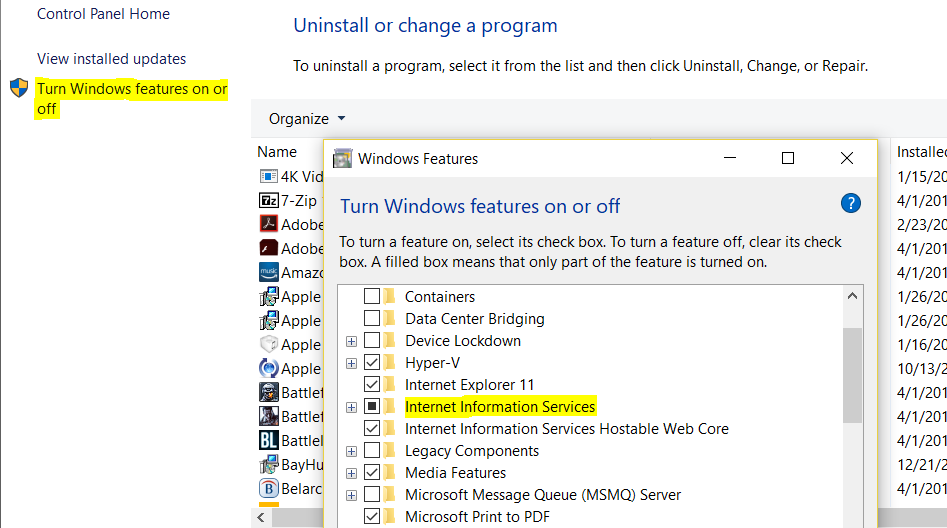
\includegraphics[width=1.0\linewidth]{Enable-IIS}
	\caption {Enabling Internet Information Services (IIS) in Windows}
	\label{fig:enable_iis}
	\vspace{-10pt}
  \end{figure}
  \begin{figure}[H]
	\centering
	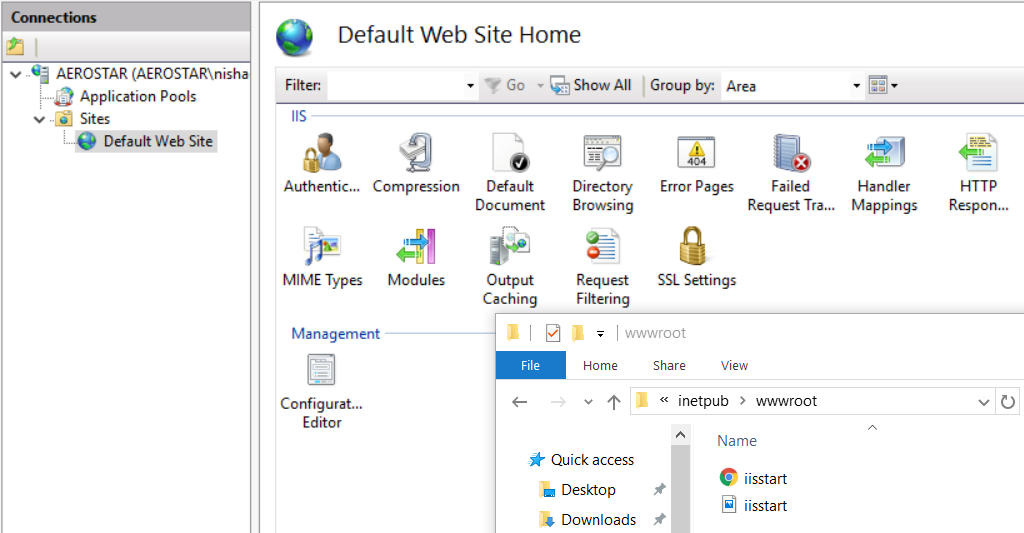
\includegraphics[width=1.0\linewidth]{IIS-www}
	\caption {IIS Server options and root directory}
	\label{fig:iis-www}
	\vspace{-10pt}
  \end{figure}
\subsection{Associating Two Mobile Clients to Access Point}
To test the handling capability of the user segregation application, two mobile clients are used as mentioned previously. There are two user ids (test and radius) that are predefined in the MySQL DB which are associated to two out port ids. The users should only be logged in once after the RYU controller is started for the user segregation application to associate the users to its out port’s. The user ‘test’ is logged in via the OpenWrt ssid and the user ‘radius’ is logged in via the OpenWrt 5G ssid as seen in the figure \ref{fig:two-ssid}.
\section{RYU Controller Performance}
The performance of RYU is discussed in the following steps, starting from running the controller to the response time of handling the associated mobile clients.

The RYU controller is initialized and started using the command \textit{ryu-manager --verbose usr\_seg.py > /tmp/log 2>\&1}, the verbose output can be viewed in real time by tailing the output from the logfile using the command \textit{tail -f /tmp/log} in a separate terminal. The detailed verbose output of RYU can be accessed in the appendix named \nameref{app:ch:logs}.
 
In the OpenWrt shell, the OVS is checked if the controller is active by issuing a command in the shell terminal \textit{ovs-vsctl show}, if it shows ‘connection is true’ then the controller has access to the OVS switch. The flow table shows the current data path that is stored for each connected device and can be viewed by using the command \textit{ovs-dpctl show}, this will show the ports and its internal port id’s starting from 1 to 3 for physical ports Eth0.3 to Eth0.5.

From the testbed layout, it can be seen that the initial RADIUS requests are made by the hostapd thru the 192.168.1.1 network. Once the authentication is complete, the mobile client initiates a DHCP request which is captured by the RYU user segregation application. The application then instructs the OVS to associate the user client to the out port id from the MySQL DB. This can be verified in the data path that is stored in the OVS Flow Table using the command as before \textit{ovs-dpctl show}. From the output, the out port assigned for the client's MAC address can be seen.

The RYU verbose log also contains this information when the user segregation application initiates the instruction to change the flow for the client. The log is documented in the appendix which can be access here \nameref{app:sec:RYUlogtrace}
%\begin{itemize}
%	\item  The RYU controller is initialized and started using the command \textit{ryu-manager --verbose usr\_seg.py > /tmp/log 2>\&1}, the verbose output can be viewed in real time by tailing the output from the logfile using the command \textit{tail -f /tmp/log} in a separate terminal. The detailed verbose output of RYU can be accessed in the appendix named \nameref{app:ch:logs}.
%	\item In the OpenWrt shell, the OVS is checked if the controller is active by issuing a command in the shell terminal \textit{ovs-vsctl show}, if it shows ‘connection is true’ then the controller as access to the OVS switch.
%	\item Now, the flow table can be viewed by using the command \textit{ovs-dpctl show}, this will show the ports and its internal port id’s starting from 1 to 3 for physical ports Eth0.3 to Eth0.5.
%	\item From the testbed layout, it can be seen that the initial RADIUS requests are made by the hostapd thru the 192.168.1.1 network. 
%	\item Once the authentication is complete, the mobile client initiates a DHCP request which is captured by the RYU user segregation application. The application then instructs the OVS to associate the user client to the out port id from the MySQL DB. 
%	\item Meanwhile, the whole flow table can be seen in the OpenWrt shell using the command ovs-dpctl show. In the output the outport assigned to the client MAC address can be seen.
%	\item In the RYU verbose log file, the applications instructions to change the flow can also be seen for the MAC address.
%	\item From the tests, it can be concluded that the users are properly associated to their out ports and can access the corresponding test IIS server machines and that too all these happens without any delay or latency for association.
%	
%\end{itemize}
\section{Open vSwitch performance}
The performance of the Open vSwitch is tested during various load scenarios using tools such as Iperfv3 and ping times. The steps to execute the tests and also analyzing the results are discussed in detail below.

Iperf is a testing tool that provies simulated loads for testing device performance in a network. The tool can be configured to generate traffic of varying sizes. It also provides a lot of customizations for each test scenarios. The Man page for Iperf shows all the options that can be used with the tool. For this project, the default settings are used. The Iperf server is running on the IIS server machines and the Iperf client was run on both IIS server machines and the mobile client.

The two scenarios for testing considered here are:
\begin{itemize}
	\item Scenario 1: Without RYU or OpenWrt to test the standard switch capacity
	\item Scenario 2: With RYU and Open vSwitch running.
\end{itemize}

ping tests were also made keeping the same scenarios as above. The results of the Iperf tests were ploted as a graph for a better analysis and each test was made three times.
%\begin{itemize}
%	\item Iperf is a testing tool that provies simulates loads to test device perfomances in a network. The tool provides loads of varying sizes and provides a lot of customizations for each test scenarios. The Man page for Iperf shows all the options that can be used with the tool.
%	\item For this project, the default settings are used. The Iperf server is running on the IIS server machines and the Iperf client was run on both IIS server machines and the mobile client.
%	\item The two scenarios for testing considered here are:
%	\begin{itemize}
%		\item Scenario 1: Without RYU or OpenWrt to test the standard switch capacity
%		\item Scenario 2: With RYU and Open vSwitch running.
%	\end{itemize}
%	\item The ping tests were also made keeping the same scenarios as above.
%	\item The results of the Iperf tests were ploted as a graph for a better analysis and each test was made three times.
%	
%\end{itemize}
\subsection{Iperf result comparison}
The graphs below show the results of the Iperf test between the IIS server machines with and without the RYU and OVS running.

\begin{figure}[H]
	\centering
	\subfloat[Bandwidth without RYU]{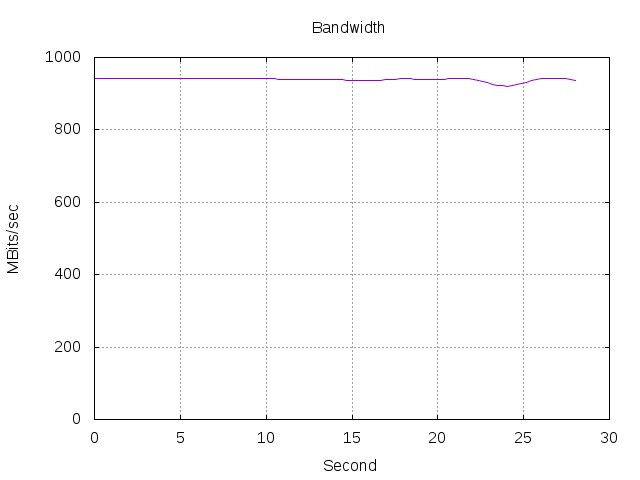
\includegraphics[width=10cm, height=10cm,keepaspectratio]{Bandwidth-without-ryu-server-server}\label{fig:bandwidth_server_server_no_ryu}}
	\hfill
	\subfloat[Bandwidth with RYU]{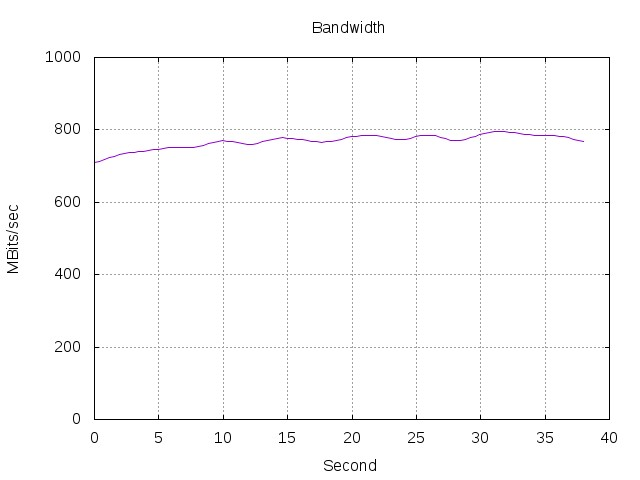
\includegraphics[width=10cm, height=10cm,keepaspectratio]{Bandwidth-with-ryu-server-server}\label{fig:bandwidth_server_server_with_ryu}}
	\caption{Iperf Throughput between two IIS servers}
\end{figure}

From the comparison, it is evident that there is a slight drop in the throughput when the RYU is running. Each ethernet port on the access point have a maximum bandwidth of 1Gbps, this is maintained when there is no RYU running on the access point. The values from the figure is shown be consistent with the maximum capacity hovering around 900Mbps. 

Whereas in the second figure, its clearly visible that the maximum achieved throughput is only available to be around 800Mbps and the waves in the graph represent the inconsistency to maintain target bandwidth.It can be concluded from this test that, running the RYU and OVS on the access point does impact the performance and bandwidth though not significantly as these speeds are still large enough to handle large traffic but with some latency.

In the next scenario, the Iperf tool is run on the mobile client and the IIS server machines though this test has a limitation. The wireless bandwidth is limited to the speeds of 802.11g and 802.11n which are mostly 54Mbps and around 100Mbps respectively. Though this test doesn’t accurately represent the capability of the RYU and OVS performance, it does show the capacity of the access point to handle through put on the wireless medium as well.

The following two figures shows the comparison of throughput bandwidth between the two scenarios.

\begin{figure}[H]
	\centering
	\subfloat[Bandwidth without RYU]{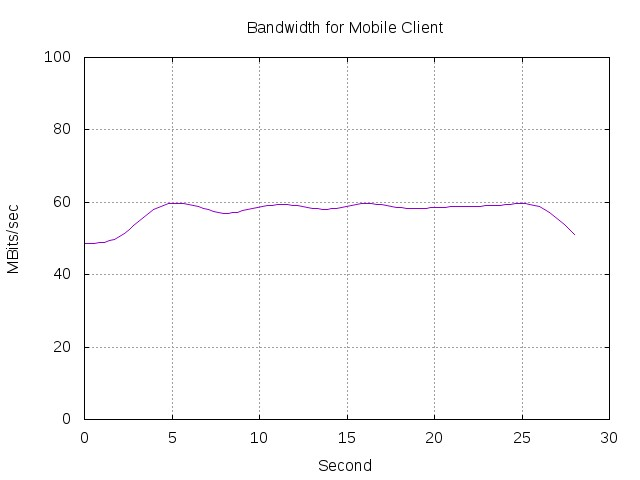
\includegraphics[width=10cm, height=10cm,keepaspectratio]{Bandwidth-without-ryu-server-client}\label{fig:bandwidth_client_server_no_ryu}}
	\hfill
	\subfloat[Bandwidth throughput with RYU]{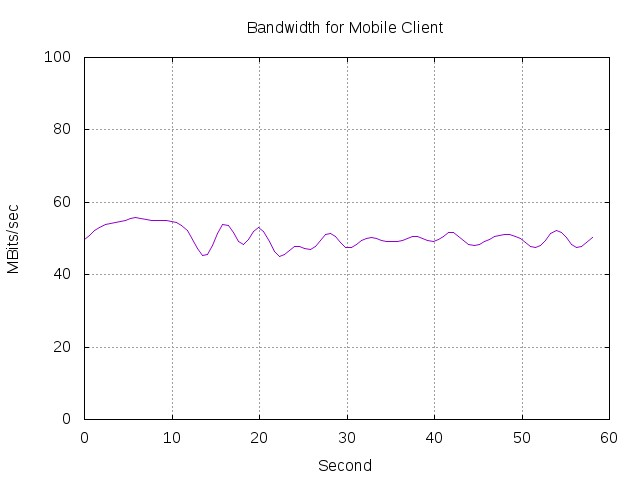
\includegraphics[width=10cm, height=10cm,keepaspectratio]{Bandwidth-with-ryu-server-client}\label{fig:bandwidth_client_server_with_ryu}}
	\caption{Iperf Throughput between Mobile client and IIS servers}
\end{figure}

The results are similar to the once above, the one without RYU and OVS seem to perform better when compared to using a RYU and OVS in the access point. As can be seen from the first graph, the bandwidth slowly starts to rise within the first 5 seconds to a maximum speed of 60Mbps which is the capacity of the wireless network. Where as in the second graph, the mobile device was only able to achieve a maximum speed of around 35 Mbps which is far below the full capacity of the wireless bandwidth and it takes more than 10 seconds to actually achieve its maximum capacity.

The initial dips are due to the wireless congestion from various other networks in the tested environment. In spite of that, the achieved bandwidth is still below the maximum capacity of the wireless network.From the above tests, it is evident that on a mobile device the impact of running RYU and OVS on the access point is more significant and can deteriorate when there is congestion in the wireless medium.

%\begin{itemize}
%	\item The graphs below show the results of the Iperf test between the IIS server machines with and without the RYU and OVS running.
%	\begin{figure}[H]
%		\centering
%		\subfloat[Bandwidth without RYU]{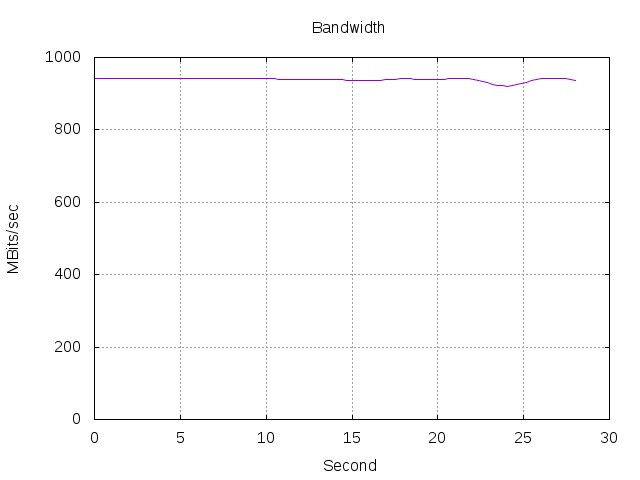
\includegraphics[width=10cm, height=10cm,keepaspectratio]{Bandwidth-without-ryu-server-server}\label{fig:bandwidth_server_server_no_ryu}}
%		\hfill
%		\subfloat[Bandwidth with RYU]{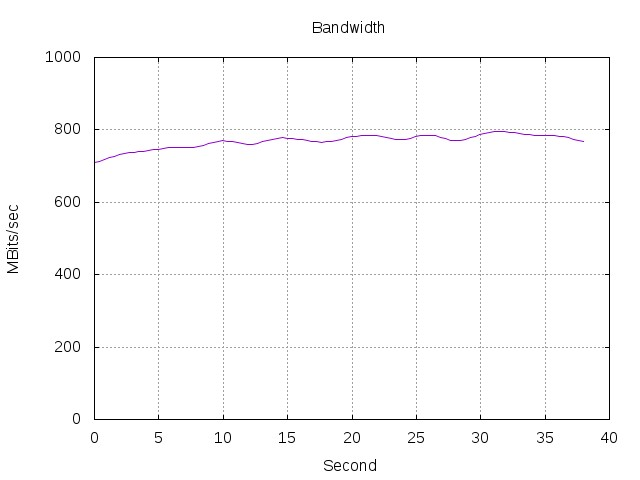
\includegraphics[width=10cm, height=10cm,keepaspectratio]{Bandwidth-with-ryu-server-server}\label{fig:bandwidth_server_server_with_ryu}}
%		\caption{Iperf Throughput between two IIS servers}
%	\end{figure}
%	\item From the comparison one can see that there is a slight drop in the throughput when the RYU is running.
%	\item Each ethernet port on the access point have a maximum bandwidth of 1Gbps, this is maintained when there is no RYU running on the access point. The values from the figure is shown be consistent with the maximum capacity hovering around 900Mbps.
%	\item Whereas in the second figure, its clearly visible that the maximum achieved throughput is only available to be around 800Mbps and the waves in the graph represent the inconsistency to maintain target bandwidth.
%	\item It can be concluded from this test that, running the RYU and OVS on the access point does impact the performance and bandwidth though not significantly as these speeds are still large enough to handle large traffic but with some latency.
%	\item In the next scenario, the Iperf tool is run on the mobile client and the IIS server machines though this test has a limitation. The wireless bandwidth is limited to the speeds of 802.11g and 802.11n which are mostly 54Mbps and around 100Mbps respectively.
%	\item Though this test doesn’t accurately represent the capability of the RYU and OVS performance, it does show the capacity of the access point to handle through put on the wireless medium as well.
%	\item The following two figures shows the comparison of throughput bandwidth between the two scenarios.
%	\begin{figure}[H]
%		\centering
%		\subfloat[Bandwidth without RYU]{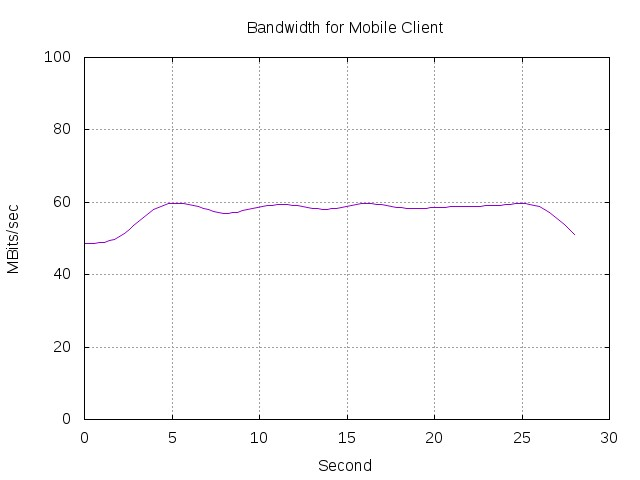
\includegraphics[width=10cm, height=10cm,keepaspectratio]{Bandwidth-without-ryu-server-client}\label{fig:bandwidth_client_server_no_ryu}}
%		\hfill
%		\subfloat[Bandwidth throughput with RYU]{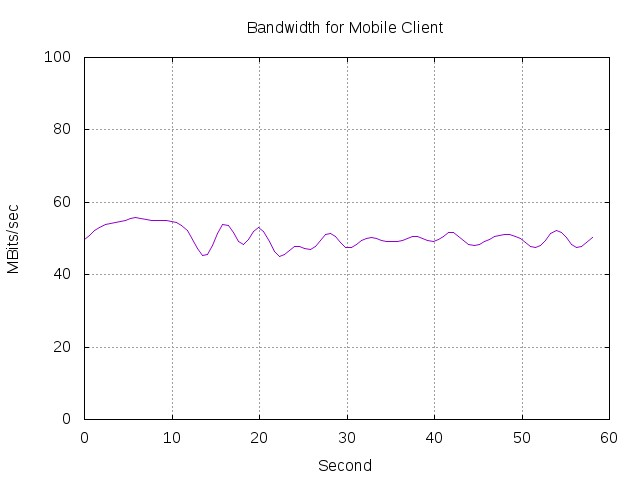
\includegraphics[width=10cm, height=10cm,keepaspectratio]{Bandwidth-with-ryu-server-client}\label{fig:bandwidth_client_server_with_ryu}}
%		\caption{Iperf Throughput between Mobile client and IIS servers}
%	\end{figure}
%	\item The results are similar to the once above, the one without RYU and OVS seem to perform better when compared to using a RYU and OVS in the access point. 
%	\item As can be seen from the first graph, the bandwidth slowly starts to rise within the first 5 seconds to a maximum speed of 60Mbps which is the capacity of the wireless network. Where as in the second graph, the mobile device was only able to achieve a maximum speed of around 35 Mbps which is far below the full capacity of the wireless bandwidth and it takes more than 10 seconds to actually achieve its maximum capacity. 
%	\item The initial dips are due to the wireless congestion from various other networks in the tested environment. In spite of that, the achieved bandwidth is still below the maximum capacity of the wireless network.
%	\item From the above tests, it is evident that on a mobile device the impact of running RYU and OVS on the access point is more significant and can deteriorate when there is congestion in the wireless medium.
%	\item On the whole, the user segregation application performs as designed and the throughput is not impacted drastically on the physical ports but the same cannot be said with the wireless network.
%	
%\end{itemize}
\subsection{Ping tests}
Ping tests provides an insight into the latency introduced due to various other activities performed by the network interfaces when a device get connected to the network from the first ping for ARP to subsequent pings.

The ping tests were executed in two methods, one is a normal test and the other is to flood. They were performed in the same scenarios used for the previous tests.

The normal results of the ping test in both the scenarios is shown below.
\begin{lstlisting}[caption={Ping Test Without OVS}, label={pingtest_no_ovs}]
--- 192.168.1.126 ping statistics ---
10 packets transmitted, 10 received, 0% packet loss, time 9197ms
rtt min/avg/max/mdev = 0.141/0.291/0.354/0.058 ms
\end{lstlisting}

\begin{lstlisting}[caption={Ping Test With OVS}, label={pingtest_ovs}]
--- 192.168.3.126 ping statistics ---
10 packets transmitted, 10 received, 0% packet loss, time 9205ms
rtt min/avg/max/mdev = 0.273/0.313/0.343/0.028 ms
\end{lstlisting}
From the result, it can be noticed that the average time is around 0.291 milliseconds when there is no OVS installed and when the OVS is running, the average is around 0.313 milliseconds. It can be inferred that there is only a slight latency between the two scenarios and that the OVS does impact a little in this regard. Though this will not be a major concern for a few devices but in a large network, this reduction in latency can impact greatly when many number of devices are connected to the access point bringing down the efficiency of the network. The results are similar when tested by ping flood. The results are shown below.

\begin{lstlisting}[caption={Ping Flood Without OVS}, label={pingflood_no_ovs}]
--- 192.168.1.126 ping statistics ---
100000 packets transmitted, 100000 received, 0% packet loss, time 18625ms
rtt min/avg/max/mdev = 0.061/0.180/51.981/0.450 ms, pipe 4, ipg/ewma 0.186/0.134 ms
\end{lstlisting}

\begin{lstlisting}[caption={Ping Flood With OVS}, label={pingflood_ovs}]
--- 192.168.3.126 ping statistics ---
100000 packets transmitted, 100000 received, 0% packet loss, time 21643ms
rtt min/avg/max/mdev = 0.111/0.205/48.572/0.526 ms, pipe 4, ipg/ewma 0.216/0.196 ms
\end{lstlisting}

The average round trip time for flood statistics in both the scenarios show that running the OVS only creates a 0.1 millisecond delay but overall for transmitting 100000 packets, it took around 3000 milliseconds more. The results are conclusive as with the previous test and demonstrates the significant increase in latency in a high traffic environment.
